\section{Total wire current}\label{sec:current}

The theory of Clements and Smy establishes that the saturation current on a wire per area, $J$, is a function of the wire diameter, $D_w$, the fluid velocity, $U$, and the ion density, $n$.  If $J_D$ were defined to represent the saturation current per unit surface area a wire of diameter $D$ would experience, then it is only a function of local ion density and bulk velocity.  In this way, $J_D$ is a locally defined fluid property from which the ion density may be deduced.  Clearly, $J_D$ is only a well defined property provided that all length scales of interest are larger than the diameter of the wire.

The value of $J_D$ is readily measured directly by insertion of a wire into the fluid.  When the fluid is uniform, the current measured, $I$, will be given by
\begin{align}
I = \pi D_w L J_D\nonumber
\end{align}
when $L$ is the length of wire inserted into the plasma.  This is the method used by MacLatchey \cite{}.

However, when the fluid is not uniform, a more sophisticated formulation is required.  In general, $J_D$ is a function in three dimensions; $x$ and $y$ perpendicular to the bulk velocity, and $z$ parallel to the direction of flow.  For the present work, we are entirely concerned with discerning the values of $J_D$ in the $x-y$ plane (for a single value of $z$ at a time).  The method we establish here may be repeated at different values of $z$ to produce complete three-dimensional maps for $J_D$.

Therefore, we may write, with sufficient generality for our needs, that
\begin{align}
I = \pi D_w \int_0^R J_D(\vec{p}(r)) \mathrm{d} r\label{eqn:I}
\end{align}
when $R$ is the radius of the spinning wire from the center of rotation, $\mathrm{d}r$ is the differential length along that radius, and $\vec{p}$ is a point along the path and an implicit function of $r$.  

Inspection of Equation \ref{eqn:I} is sufficient to conclude that a single measurement of $I$ cannot distinguish between an infinite number of possible spatial distributions of $J_D$.  Instead, it should be possible to deduce a specific $J_D$ map by collecting a series of overlapping but dissimilar trajectories for the wire in $x$-$y$ space.

As shown in Figure \ref{fig:coordinate}, a spinning disc with a wire probe could be passed through a flame with varying depths.  When only the tip of the wire interacts with the flame, it would be certain that any electrical currents were collected at the wire's tip.  Successively deeper passes through the flame could benefit from the prior measurements by subtracting the already known currents to infer the new currents realized at the wire's tip. 

\begin{figure}
\begin{center}
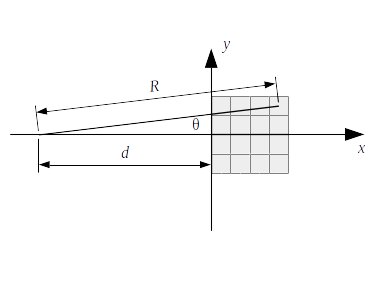
\includegraphics{coordinates}
\caption{The measurement coordinate system with the measurement region shown in gray.}\label{fig:coordinate}
\end{center}
\end{figure}

This approach would be akin to the Abel transformation used to infer an axis-symmetric quantity from a plurality of line-of-sight integrated measurements.  However, there are a number of issues that plague a straight-forward application of the method as described.  In order to evaluate the integral in Equation \ref{eqn:I}, it will become necessary to interpolate between the prior results of current measurements that will not lie precisely on the line formed by the wire.  This calls for an interpolation scheme, but it is not immediately obvious what artifacts may be introduced by such a method.  It seems likely that small errors will accumulate from shallower measurements so that the deeper ones may suffer undesirable uncertainties.

Instead, we will adopt a more general problem: what field values of $J_D(x,y)$ minimize the error between many individual wire current measurements and wire currents calculated from the $J_D(x,y)$ field?  While this preliminary statement makes no presumption on how the wire measurements were taken, as we see in Figure \ref{fig:coordinate}, wire current, $I(s,\theta)$, can be said to be a function of the center of rotation and the disc's angle.  The fundamental problem is to calculate field values for $J_D$ from many values of $I$.  This approach takes advantage of how easily $I$ can be calculated from $J_D$, makes no presumption that the signals are free of noise, and permits a disorganized cloud of individual measurements.

The error due to each measurement, $I_k(s_k, \theta_k)$, may be calculated
\begin{align}
e_k &= - I_k\left(s_k, \theta_k\right) + \pi D_w \int_0^R J_D\left(\vec{p}_k(r)\right) \mathrm{d} r\label{eqn:ek}\\
\vec{p}_k(r) &= [x_k(r),\ y_k(r)]^T = [-s_k + r\cos(\theta_k),\ r\sin(\theta_k)]^T \nonumber
\end{align}
When we use the method of least squares, we obtain a total error metric
\begin{align}
E^2 = \sum_k e_k{^2}.
\end{align}
Now, we turn our attention to how the field of values for $J_D$ should be constructed.
